\documentclass{article}
\usepackage{eecstex}
\usepackage{pgfplots}

\renewcommand{\thesubsection}{\thesection.\arabic{subsection}}
\renewcommand{\thesubsubsection}{\thesubsection.\alph{subsubsection}}
\renewcommand{\labelenumi}{\arabic{enumi}.}
\newcommand{\F}{\mathcal{F}}
\newcommand{\sinc}{\operatorname{sinc}}
\newcommand{\rect}{\operatorname{rect}}


\title{EE 120 HW 09}
\author{Bryan Ngo}
\date{2021-03-28}

\begin{document}

\maketitle

\section{2D Filter}

\subsection{}

\begin{equation}
    h[n_1, n_2] = \frac{1}{5} (\delta[n_1, n_2] + \delta[n_1 - 1, n_2] + \delta[n_1 + 1, n_2] + \delta[n_1, n_2 - 1] + \delta[n_1, n_2 + 1])
\end{equation}

\subsection{}

Note that
\begin{align}
    h[n_1, n_2] &= \frac{1}{5} (\delta[n_1] \delta[n_2] + \delta[n_1 - 1] \delta[n_2] + \delta[n_1 + 1] \delta[n_2] + \delta[n_1] \delta[n_2 - 1] + \delta[n_1] \delta[n_2 + 1]) \\
    H(e^{j \omega_1}, e^{j \omega_2}) &= \frac{1}{5} (1 + e^{-j \omega_1} + e^{j \omega_1} + e^{-j \omega_2} + e^{j \omega_2}) == \frac{1}{5} (1 + 2\cos(\omega_1) + 2\cos(\omega_2)) \\
    |H(e^{j \omega_1}, e^{j \omega_2}) &= \frac{1}{5} (1 + 2|\cos(\omega_1)| + 2|\cos(\omega_2)|)
\end{align}
where we use the linearity and separation property of the 2D DTFT.

\begin{center}
    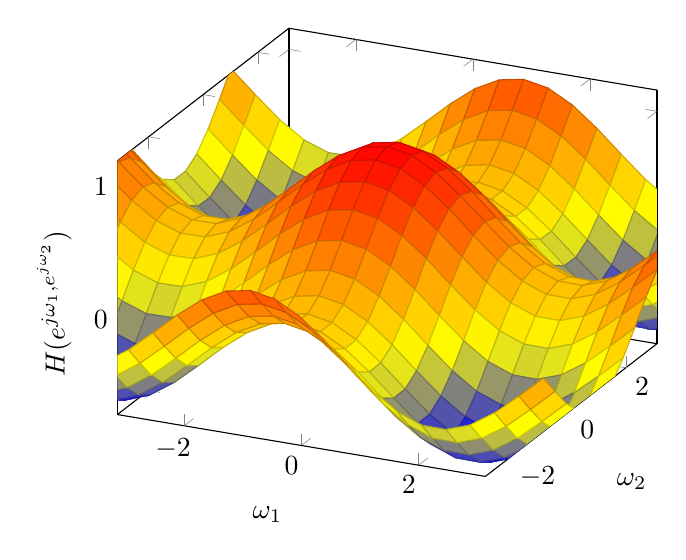
\begin{tikzpicture}
        \begin{axis}[
            xlabel=\(\omega_1\),
            ylabel={\(\omega_2\)},
            zlabel={\(H(e^{j \omega_1, e^{j \omega_2}})\)},
            xmin=-pi, xmax=pi,
            ymin=-pi, ymax=pi,
        ]
        \addplot3[
            surf,
        ]
        {(1 + 2 * cos(deg(x)) + 2 * cos(deg(y))) / 5};
        \end{axis}
    \end{tikzpicture}
    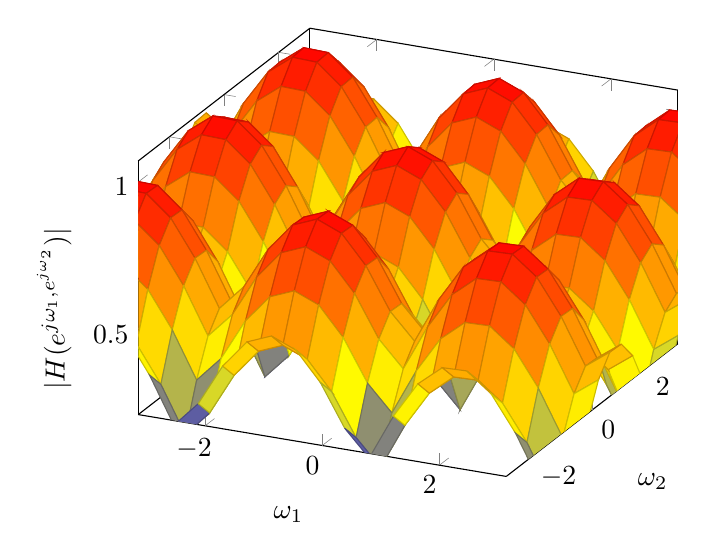
\begin{tikzpicture}
        \begin{axis}[
            xlabel=\(\omega_1\),
            ylabel={\(\omega_2\)},
            zlabel={\(|H(e^{j \omega_1, e^{j \omega_2}})|\)},
            xmin=-pi, xmax=pi,
            ymin=-pi, ymax=pi,
        ]
        \addplot3[
            surf,
        ]
        {(1 + 2 * abs(cos(deg(x))) + 2 * abs(cos(deg(y)))) / 5};
        \end{axis}
    \end{tikzpicture}
\end{center}

\section{FIR Filter}

\begin{equation}
    a[n] = \sum_{k \in [0, N]} a_k \delta[n - k]
\end{equation}

\subsection{}

By linearity of the CTFT,
\begin{equation}
    A(\omega) = \sum_{k \in [0, N]} a_k e^{-j \omega k}
\end{equation}
where the coefficients are the same as \(a[n]\).

\subsection{}

\begin{enumerate}
    \item \(c[n] = (a \ast b)[n]\)
    \item \(C(e^{j \omega}) = A(e^{j \omega}) B(e^{j \omega})\)
    \item Since \(C\) is going to be a product of 2 polynomials, the result is going to be another polynomial in terms of \(e^{-j \omega}\), meaning its inverse CTFT will be in the form of an FIR filter with new coefficients.
\end{enumerate}

\subsection{}

We can express the polynomial multiplication as
\begin{equation}
    C(z) = \sum_{i \in [0, N]} \sum_{j \in [0, M]} a_i b_j z^i z^j
\end{equation}
Letting \(k = i + j\),
\begin{align}
    C(z) &= \sum_{i \in [0, N]} \sum_{j \in [0, M]} a_i b_{k - i} x^k \\
    &= \sum_{k \in [0, N + M]} \sum_{i + j = k} a_i b_j x^k \\
    &= \sum_{k \in [0, N + M]} \underbrace{\sum_{i \in [0, k]} a_i b_{k - i}}_{c_n} x^k
\end{align}
where we have found the coefficients in terms of a convolution.

\section{Sampling Basics}

\begin{align}
    x_p(t) &= x(t) p(t) \\
    p(t) &= \sum_{k \in \Z} \delta(t - kT)
\end{align}

\subsection{}

The minimum sampling rate is \SI{13}{\kilo\hertz}, which is a quarter of the Nyquist frequency.

\subsection{}



\end{document}
